\documentclass{article}
\begin{document}
\section{Using Sensor API with COINES}
\subsection{SensorAPI}
Bosch Sensortec recommends using the SensorAPI in order to communicate with the sensors. The SensorAPI, an abstraction layer written in C makes it much more convenient for the user to access the register map of the sensor, in order to configure certain functionality and obtain certain information from it.

For making use of the SensorAPI, some function pointers must be set to the appropriate read/write functions of the selected bus on the system (either I\textsuperscript{2}C or SPI), as well as one function pointer to a system's function causing delays in milliseconds.

In order to execute C code using SensorAPI, the COINES API provides the mentioned read, write, delay functions. These functions are wrapper functions, embedding the actual SensorAPI payloads into a transport package, sending this via USB or BLE to the Engineering board, where the payload is translated into corresponding SPI or I\textsuperscript{2}C messages and sent to the sensor on the shuttle board.The mapping would look similar to the one below.

\begin{lstlisting}
#include "coines.h"
#include "bst_sensor.h"

struct bst_sensor_dev sensordev;
....
....
sensordev.intf = BST_SENSOR_I2C_INTF;  // SPI - BST_SENSOR_SPI_INTF
sensordev.read = coines_read_i2c;   // coines_read_spi
sensordev.write = coines_write_i2c; // coines_write_spi
sensordev.delay_ms = coines_delay_usec;

\end{lstlisting}

For the description of COINES functions used, refer to \ref{CoinesCFunctions}.

\subsection{Downloading Sensor API}
In order to download SensorAPI, the steps below need to be followed:
\begin{itemize}
	\item Download SensorAPI repo using Download zip option for selected sensors from boschsensortec github \url{https://github.com/BoschSensortec}.
	\item Unzip the downloaded SensorAPI repo to \path{\examples}.
	\item Rename the unzipped folder to sensor name e.g \path{\examples\bmi270} and change directory to an example folder to execute it.
\end{itemize}

\subsection{Running example on MCU side}
Here are the step-by-step instructions to run examples on MCU side:
\begin{itemize}
	\item Selected Platform: Windows
	\item Board: APP3.1
	\item Sensor shuttle: BMI270
	\item Example: \path{\examples\bmi270\bmi270_examples\accel_gyro}
\end{itemize}
\begin{enumerate}
	\item Connect the Application Board board via USB, with the sensor shuttle board mounted.
	\item Open the command prompt or the terminal.
	\item Use the command \texttt{cd} to go to the directory where the example that is to be built is located.
	\begin{figure}[H]
		\begin{center}
			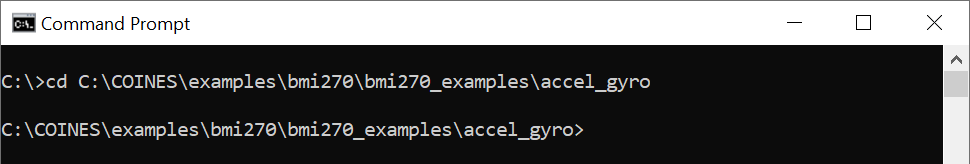
\includegraphics[width=0.9\textwidth]{coinesAPI_images/Mcu_example_cd.png}
		\end{center}
	\end{figure}
	\item Execute command "mingw32-make TARGET=MCU\_APP31 download"
	\begin{figure}[H]
		\begin{center}
			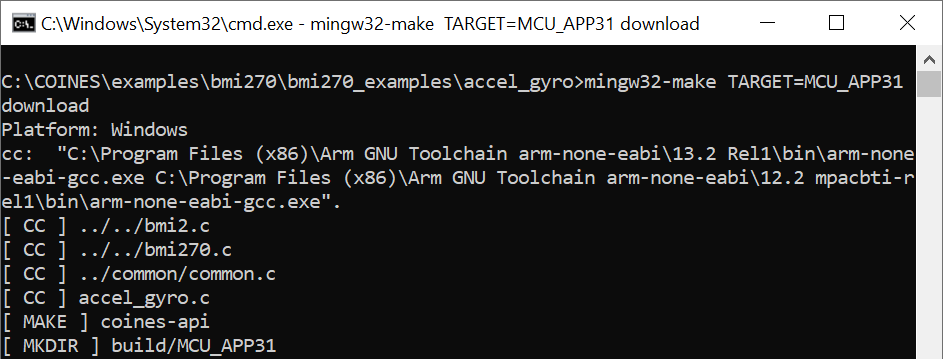
\includegraphics[width=0.9\textwidth]{coinesAPI_images/Mcu_example_compile.png}
		\end{center}
	\end{figure}
	\begin{figure}[H]
		\begin{center}
			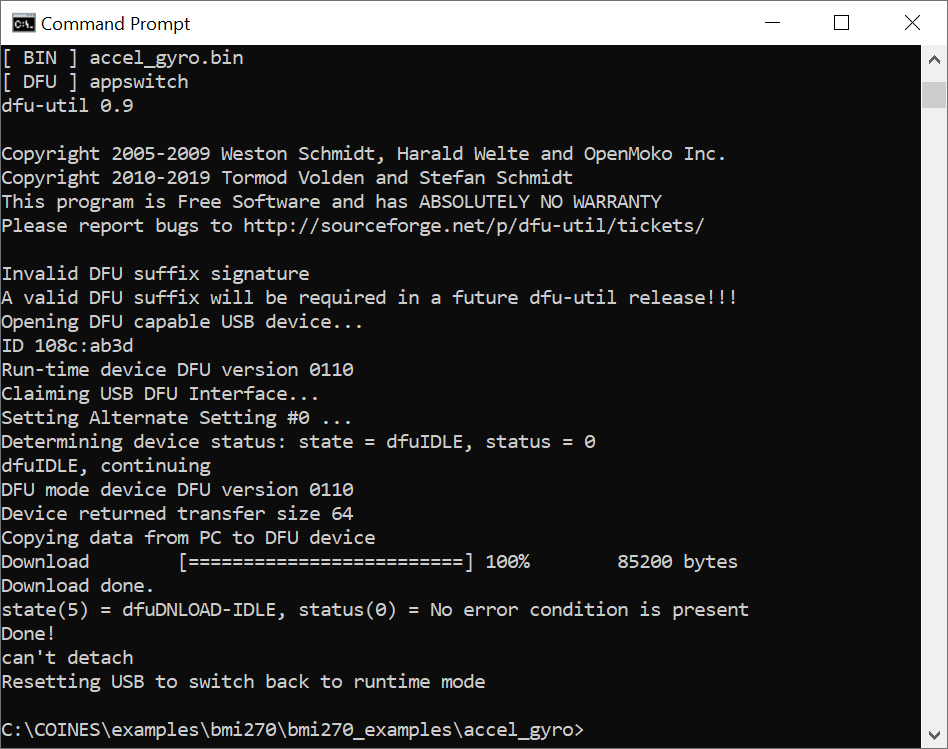
\includegraphics[width=0.9\textwidth]{coinesAPI_images/Mcu_example_download.png}
		\end{center}
	\end{figure}
	\item View the output in a serial terminal application like HTerm
	\begin{figure}[H]
		\begin{center}
			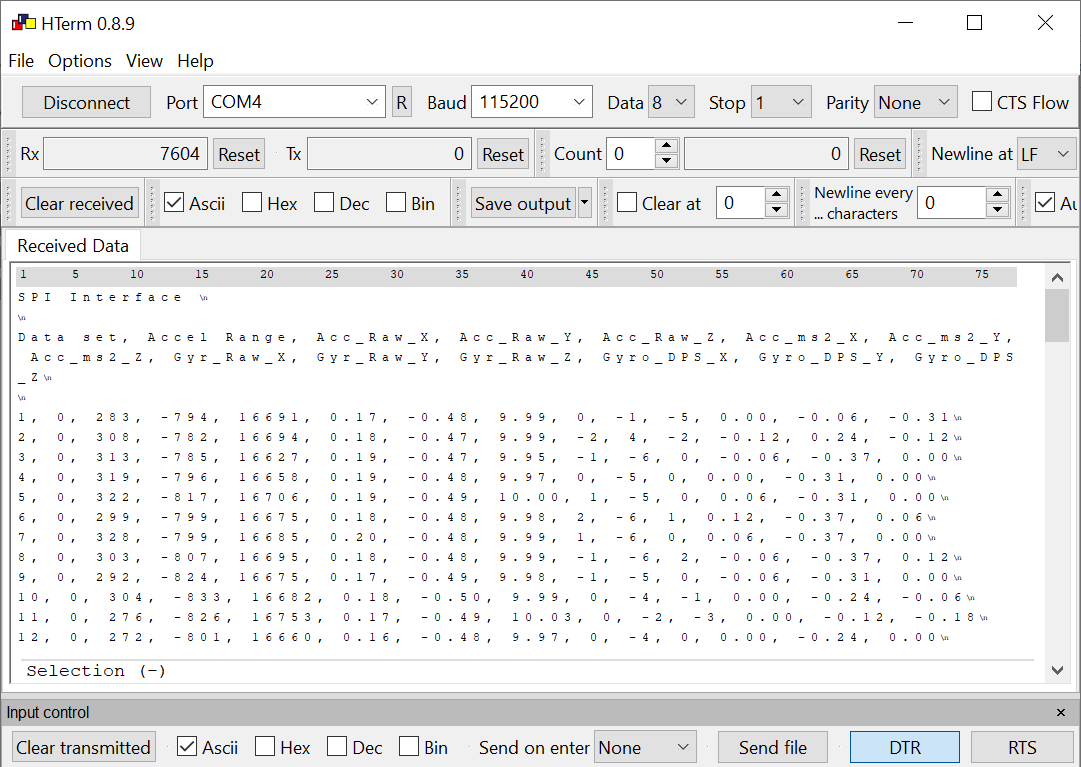
\includegraphics[width=0.9\textwidth]{coinesAPI_images/Mcu_example_output.png}
		\end{center}
	\end{figure}
	\begin{figure}[H]
		\begin{center}
			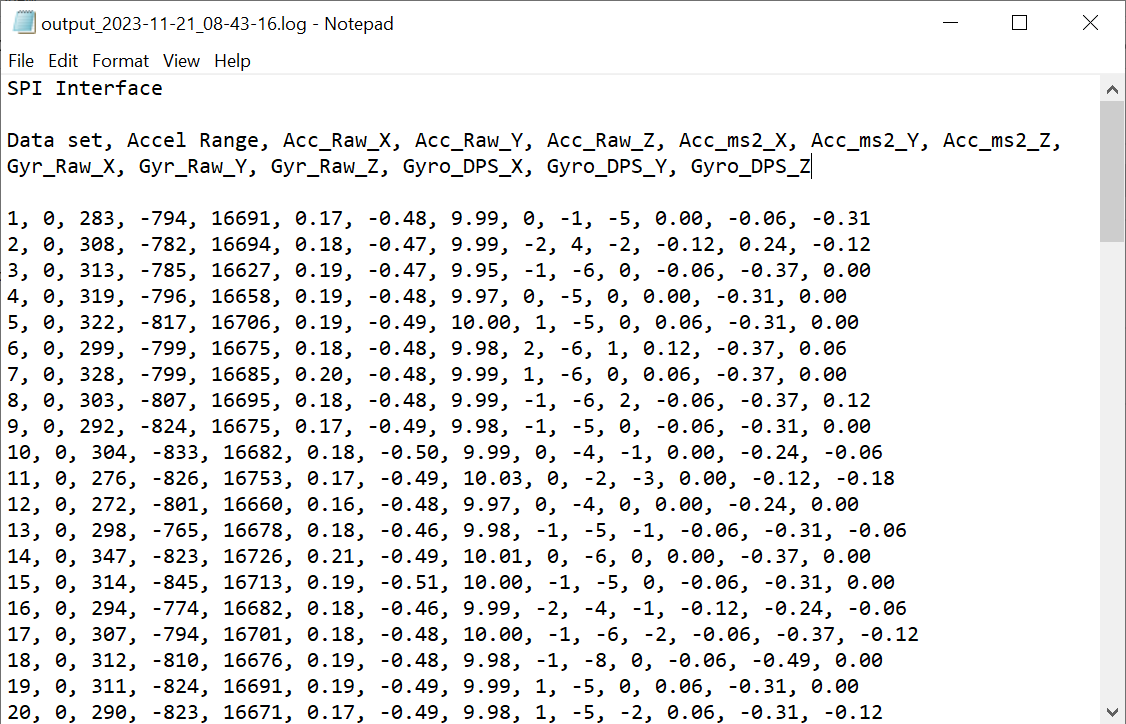
\includegraphics[width=0.9\textwidth]{coinesAPI_images/Mcu_example_log.png}
		\end{center}
	\end{figure}
\end{enumerate}
\subsection{Running example on MCU side via BLE}
The sequence of actions required for interfacing via BLE includes the steps below:
\begin{enumerate}
	\item Go to the \path{examples} folder in file explorer
	\item Open the common.c file in the selected example folder in your IDE
	\item Change COINES\_COMM\_INTF\_USB  to COINES\_COMM\_INTF\_BLE
	\begin{figure}[H]
		\begin{center}
			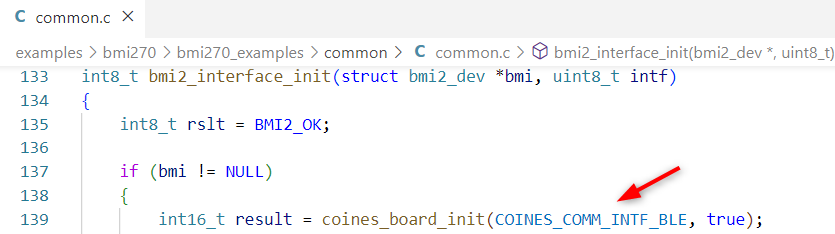
\includegraphics[width=0.9\textwidth]{coinesAPI_images/Mcu_example_ble_intf.png}
		\end{center}
	\end{figure}
	\item Open example script and change the 
	\begin{verbatim}
	printf(...) to fprintf(bt_w,...)
	\end{verbatim}
	\begin{figure}[H]
		\begin{center}
			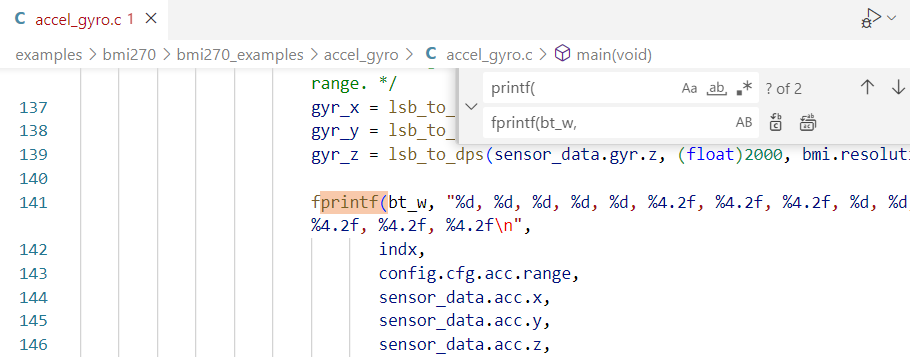
\includegraphics[width=0.9\textwidth]{coinesAPI_images/Mcu_example_ble_print.png}
		\end{center}
	\end{figure}
	\item Now follow the same steps from 1 - 4 in the above section.
	\item Connect the Application board to another power source and keep it within the BLE range.
	\item View the output in the \href{https://wiki.makerdiary.com/web-device-cli/}{Web Device CLI} site in your browser by connecting to board via BLE.
	\begin{figure}[H]
		\begin{center}
			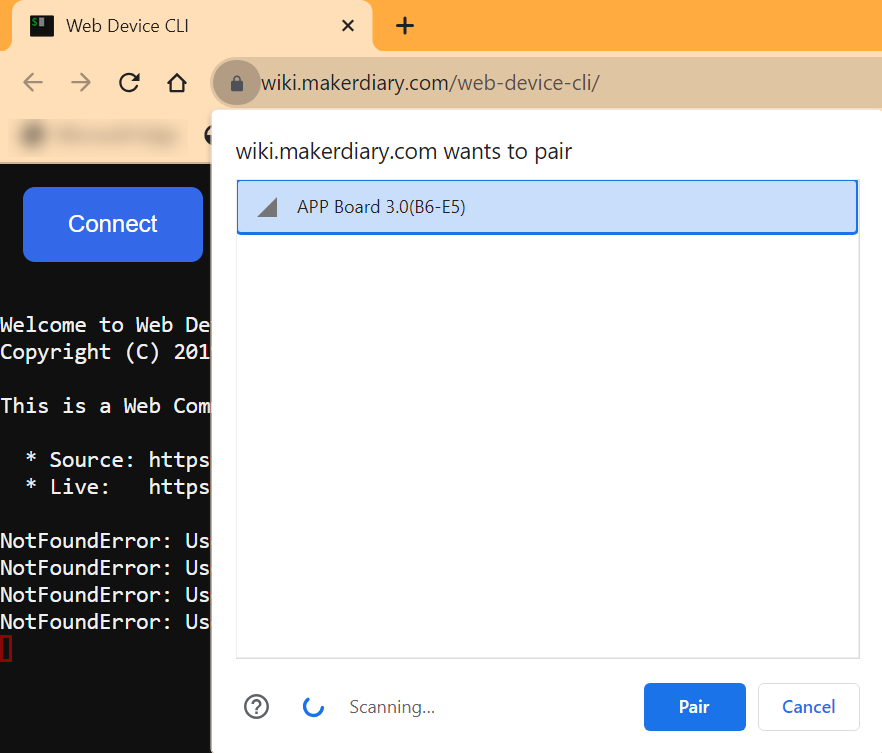
\includegraphics[width=0.7\textwidth]{coinesAPI_images/Mcu_example_ble_pair.png}
		\end{center}
	\end{figure}
	\begin{figure}[H]
		\begin{center}
			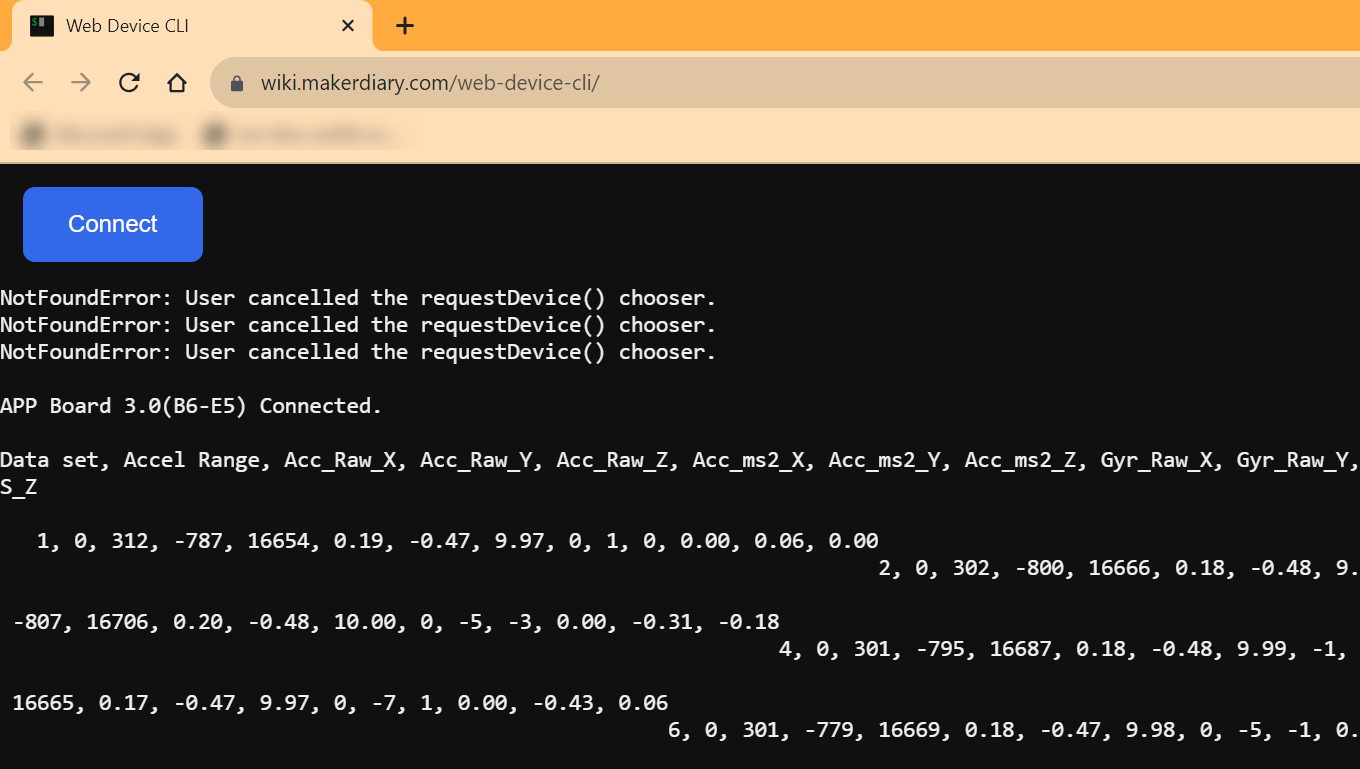
\includegraphics[width=0.9\textwidth]{coinesAPI_images/Mcu_example_ble_output.png}
		\end{center}
	\end{figure}
\end{enumerate}


\subsection{Running example on PC side}
Here are the step-by-step instructions to run examples on PC side:
\begin{itemize}
	\item Selected Platform: Windows
	\item Board: APP3.1
	\item Sensor shuttle: BMI270
	\item Example: \path{\examples\bmi270\bmi270_examples\step_counter}
\end{itemize}
\begin{enumerate}
	\item Connect the Application Board board via USB, with the sensor shuttle board mounted.
	\item Refer to section \ref{firmwareUpdate} and update the Coines Bridge firmware to the board.
	\item Open the command prompt or the terminal.
	\item Use the command \texttt{cd} to go to the directory where the example that is to be built is located.
	\begin{figure}[H]
		\begin{center}
			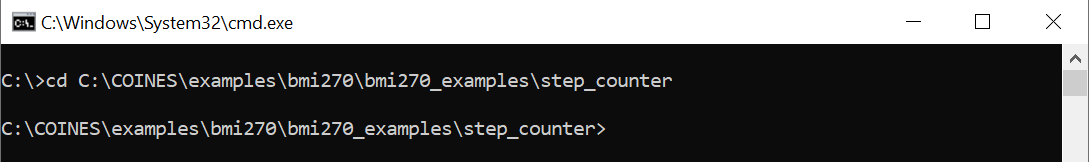
\includegraphics[width=0.9\textwidth]{coinesAPI_images/Pc_example_cd.png}
		\end{center}
	\end{figure}
	\item Execute command "mingw32-make TARGET=PC COINES\_BACKEND=COINES\_BRIDGE"
	\begin{figure}[H]
		\begin{center}
			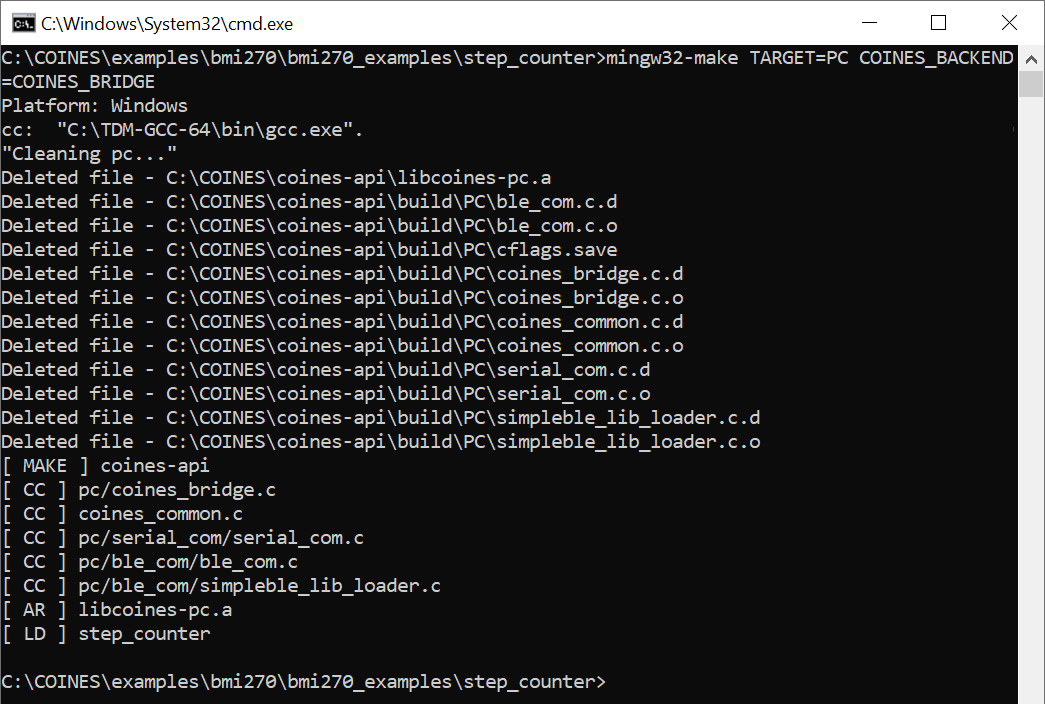
\includegraphics[width=0.9\textwidth]{coinesAPI_images/Pc_example_compile.png}
		\end{center}
	\end{figure}
	\item View the output in the command prompt by running the example executable.
	\begin{figure}[H]
		\begin{center}
			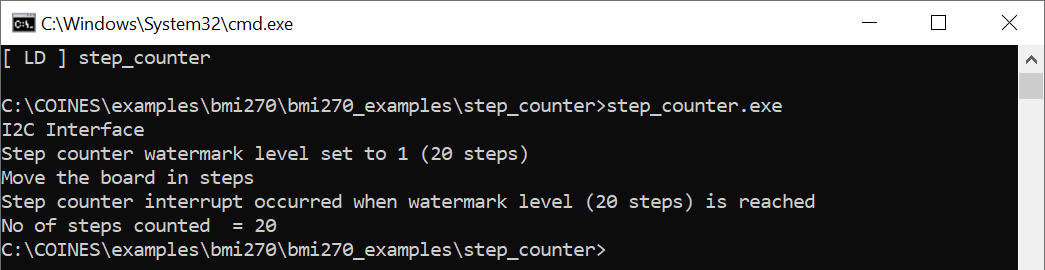
\includegraphics[width=0.9\textwidth]{coinesAPI_images/Pc_example_output.png}
		\end{center}
	\end{figure}
\end{enumerate}

\subsection{Running example on PC side via BLE}
The sequence of actions required for interfacing via BLE includes the steps below:
\begin{enumerate}
	\item Go to the examples folder in file explorer.
	\item Open the common.c file in the selected example folder in your IDE.
	\item Change COINES\_COMM\_INTF\_USB  to COINES\_COMM\_INTF\_BLE.
	\item Connect the Application board to another power source and keep it within the BLE range.
	\item Now follow the same steps from 3 - 6 in the above section.
	\begin{figure}[H]
		\begin{center}
			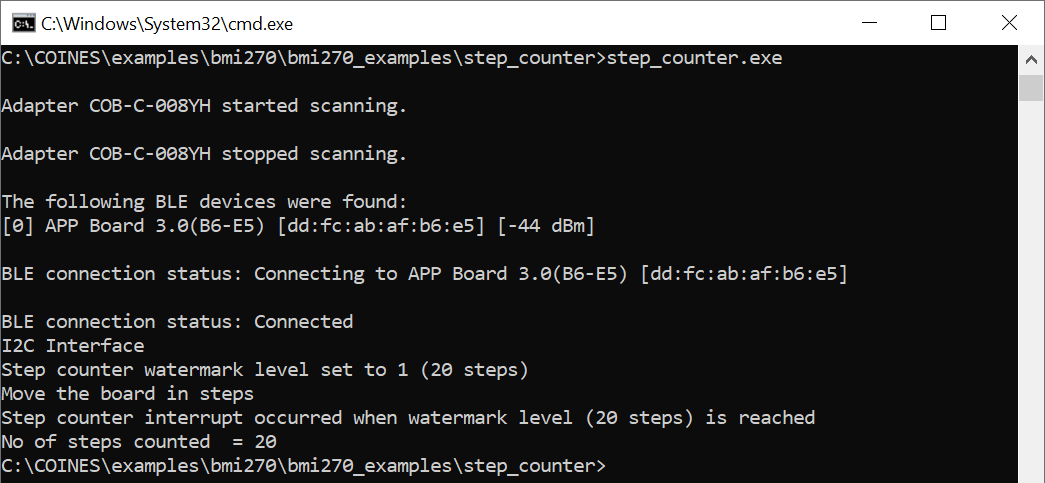
\includegraphics[width=0.9\textwidth]{coinesAPI_images/Pc_example_ble_output.png}
		\end{center}
	\end{figure}
\end{enumerate}
\newpage

\end{document}